\chapter{玻色化}

\section{一维电子系统的玻色化}

任何电子系统都可以展现出密度波,即$\expval*{{c}^\dagger {c}}$的长程序。实际上,一维电子系统可以完全使用它的密度波和与之紧密相关的另一个场来描述。
这意味着电子系统的低能激发实际上未必总是“重整化之后的电子”——它甚至可以是玻色子!

物理地说,这是因为一维电子系统中,一个电子不能“绕过”另一个电子,从而稍许相互作用就足够造成非常明显的密度波——或是别的什么波——的涨落。
一维电子系统生来就是强关联的。

本节暂时忽略一维电子系统的自旋,或者,等价地说,假定不存在任何区分两个自旋的过程。

\subsection{费米点附近的有效理论}

\begin{figure}
    \centering
    
    \tikzset{every picture/.style={line width=0.75pt}} %set default line width to 0.75pt        

    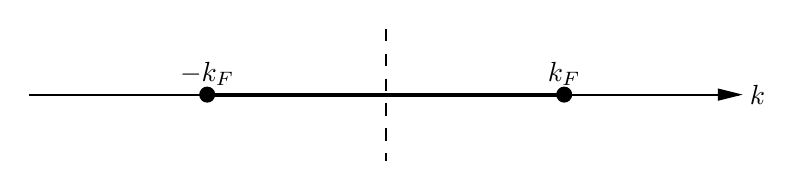
\begin{tikzpicture}[x=0.75pt,y=0.75pt,yscale=-1,xscale=1]
    %uncomment if require: \path (0,171); %set diagram left start at 0, and has height of 171

    %Straight Lines [id:da16577971185477902] 
    \draw    (100,114) -- (272,114) ;
    %Straight Lines [id:da2853357697117014] 
    \draw    (272,114) -- (442,114) ;
    \draw [shift={(444,114)}, rotate = 180] [fill={rgb, 255:red, 0; green, 0; blue, 0 }  ][line width=0.08]  [draw opacity=0] (12,-3) -- (0,0) -- (12,3) -- cycle    ;
    %Straight Lines [id:da28061773936940027] 
    \draw [line width=1.5]    (186,114) -- (358,114) ;
    %Straight Lines [id:da638769097798594] 
    \draw  [dash pattern={on 4.5pt off 4.5pt}]  (272,82.25) -- (272,145.75) ;
    %Straight Lines [id:da24278605860678137] 
    \draw    (186,114) ;
    \draw [shift={(186,114)}, rotate = 0] [color={rgb, 255:red, 0; green, 0; blue, 0 }  ][fill={rgb, 255:red, 0; green, 0; blue, 0 }  ][line width=0.75]      (0, 0) circle [x radius= 3.35, y radius= 3.35]   ;
    %Straight Lines [id:da5286794669194295] 
    \draw    (358,114) ;
    \draw [shift={(358,114)}, rotate = 0] [color={rgb, 255:red, 0; green, 0; blue, 0 }  ][fill={rgb, 255:red, 0; green, 0; blue, 0 }  ][line width=0.75]      (0, 0) circle [x radius= 3.35, y radius= 3.35]   ;

    % Text Node
    \draw (446,114) node [anchor=west] [inner sep=0.75pt]    {$k$};
    % Text Node
    \draw (358,111) node [anchor=south] [inner sep=0.75pt]    {$k_{\text{F}}$};
    % Text Node
    \draw (186,111) node [anchor=south] [inner sep=0.75pt]    {$-k_{\text{F}}$};


    \end{tikzpicture}
    \caption{一维系统的动量空间,描黑的部分是一维费米“球”}
    \label{fig:one-dim-moment-space}
\end{figure}

考虑一个一维近独立电子系统。
一维系统的动量只有一个可能的方向。因此,一维系统的费米面无非是两个\concept{费米点}。由对称性这两个点距离动量原点的位置是相同的。
动量空间的情况展示如\autoref{fig:one-dim-moment-space},其中描黑的部分是一维费米“球”。

考虑费米点附近的能量,做线性近似,有
\begin{equation}
    \xi_{k} = \pm v_\text{F} (k - k_\text{F}).
\end{equation}
方程前面加正负号是因为色散关系是左右对称的,所以在两个费米点处的斜率互为相反数。
从费米面以下到费米面以上能量总是增加的,于是斜率为正表示$k>0$,斜率为负表示$k<0$。

我们将讨论费米点附近的低能有效理论,则晶格上的布洛赫产生湮灭算符中只有晶格动量集中在$\abs{k_\text{F}}$附近的部分是有意义的。
由于哈密顿量中不同动量的模式无耦合,可以直接弃去高动量模式,得到有效哈密顿量为
\[
    {H}_\text{eff} = \sum_{\text{$k$ near $\pm k_\text{F}$}} \xi_k {c}^\dagger_{k \sigma} {c}_{k \sigma} = \sum_{\text{$k$ near $k_\text{F}$}} v_\text{F} (k - k_\text{F}) {c}^\dagger_{k \sigma} {c}_{k \sigma} + \sum_{\text{$k$ near $-k_\text{F}$}} v_\text{F} ( - k - k_\text{F}) {c}^\dagger_{k \sigma} {c}_{k \sigma}  ,
\]
为了简化,记
\begin{equation}
    p = \begin{cases}
        k - k_\text{F}, \quad k > 0, \\
        k + k_\text{F} , \quad k < 0,
    \end{cases}
\end{equation}
并使用$p$来标记布洛赫模式,则
\begin{equation}
    \begin{aligned}
        {H}_\text{eff} &= \sum_{\abs{p} < \Lambda} (v_\text{F} \abs{p} {c}^\dagger_{ \text{L} p\sigma} {c}_{\text{L} p\sigma} + v_\text{F} \abs{p} {c}^\dagger_{ \text{R} p\sigma} {c}_{\text{R} p\sigma}) \\
        &= \sum_{\abs{p} < \Lambda} (v_\text{F} p {c}^\dagger_{ \text{L} p\sigma} {c}_{\text{L} p\sigma} - v_\text{F} p {c}^\dagger_{ \text{R} p\sigma} {c}_{\text{R} p\sigma}),
    \end{aligned}
\end{equation}
其中$\Lambda$是一个截断参量,R和L分别表示对应的模式在$k>0$处(称为\concept{右模式}),以及对应的模式在$k<0$处(称为\concept{左模式})。
费米海以外的右模式的$p>0$,左模式的$p < 0$。(下面会看到,这么定义是为了让以$p$为动量的对${c}_{(\text{L}, \text{R}) \sigma}$的傅里叶逆变换能够给出物理意义明确的结果)
在自由哈密顿量中不同自旋之间完全解耦,暂时只考虑一个自旋取值,于是
\begin{equation}
    {H}_\text{eff} = \sum_{\abs{p} < \Lambda} (v_\text{F} p {c}^\dagger_{\text{L} p} {c}_{\text{L} p} - v_\text{F} p {c}^\dagger_{\text{R} p} {c}_{\text{R} p}).
    \label{eq:one-dimension-linear-model}
\end{equation}
若以$p$为动量,则${c}_{\text{R} p}$在坐标空间中对应着什么?容易发现,它对应的坐标空间中的湮灭算符正是${c}_{n\sigma}$以频率$\pm k_\text{F}$在空间上振荡的振幅,即
\begin{equation}
    {c}_{n\sigma} = \ee^{\ii k_\text{F} na} {c}_{\text{R} n \sigma } + \ee^{ - \ii k_\text{F} na} {c}_{\text{L} n \sigma},
\end{equation}
它们在空间上是缓变的。% TODO:${\psi}_{\text{R}}(x)$??

\subsection{玻色化}

\begin{figure}
    \subfigure[基态]{
        

\tikzset{every picture/.style={line width=0.75pt}} %set default line width to 0.75pt        

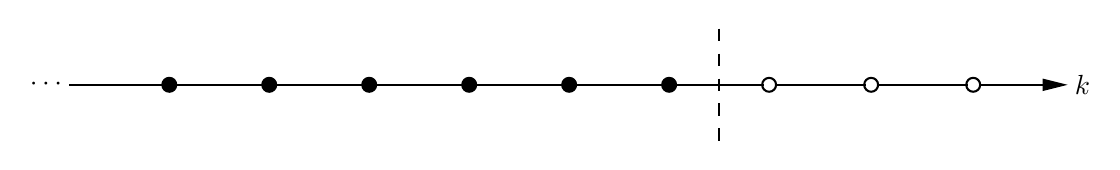
\begin{tikzpicture}[x=0.75pt,y=0.75pt,yscale=-1,xscale=1]
%uncomment if require: \path (0,300); %set diagram left start at 0, and has height of 300

%Straight Lines [id:da389985056516742] 
\draw    (100,102) -- (148.17,102) ;
\draw [shift={(148.17,102)}, rotate = 0] [color={rgb, 255:red, 0; green, 0; blue, 0 }  ][fill={rgb, 255:red, 0; green, 0; blue, 0 }  ][line width=0.75]      (0, 0) circle [x radius= 3.35, y radius= 3.35]   ;
%Straight Lines [id:da8735536812464386] 
\draw    (148.17,102) -- (196.33,102) ;
\draw [shift={(196.33,102)}, rotate = 0] [color={rgb, 255:red, 0; green, 0; blue, 0 }  ][fill={rgb, 255:red, 0; green, 0; blue, 0 }  ][line width=0.75]      (0, 0) circle [x radius= 3.35, y radius= 3.35]   ;
%Straight Lines [id:da7221208832553236] 
\draw    (196.33,102) -- (244.5,102) ;
\draw [shift={(244.5,102)}, rotate = 360] [color={rgb, 255:red, 0; green, 0; blue, 0 }  ][fill={rgb, 255:red, 0; green, 0; blue, 0 }  ][line width=0.75]      (0, 0) circle [x radius= 3.35, y radius= 3.35]   ;
%Straight Lines [id:da22657899441580232] 
\draw    (244.5,102) -- (292.67,102) ;
\draw [shift={(292.67,102)}, rotate = 0] [color={rgb, 255:red, 0; green, 0; blue, 0 }  ][fill={rgb, 255:red, 0; green, 0; blue, 0 }  ][line width=0.75]      (0, 0) circle [x radius= 3.35, y radius= 3.35]   ;
%Straight Lines [id:da055761283547104634] 
\draw    (292.67,102) -- (340.83,102) ;
\draw [shift={(340.83,102)}, rotate = 0] [color={rgb, 255:red, 0; green, 0; blue, 0 }  ][fill={rgb, 255:red, 0; green, 0; blue, 0 }  ][line width=0.75]      (0, 0) circle [x radius= 3.35, y radius= 3.35]   ;
%Straight Lines [id:da9070988727925184] 
\draw    (340.83,102) -- (389,102) ;
\draw [shift={(389,102)}, rotate = 0] [color={rgb, 255:red, 0; green, 0; blue, 0 }  ][fill={rgb, 255:red, 0; green, 0; blue, 0 }  ][line width=0.75]      (0, 0) circle [x radius= 3.35, y radius= 3.35]   ;
%Straight Lines [id:da57324706717669] 
\draw    (538.5,102) -- (579,102) ;
\draw [shift={(581,102)}, rotate = 180] [fill={rgb, 255:red, 0; green, 0; blue, 0 }  ][line width=0.08]  [draw opacity=0] (12,-3) -- (0,0) -- (12,3) -- cycle    ;
%Straight Lines [id:da567630885526011] 
\draw    (440.17,102) -- (483.98,102) ;
\draw [shift={(486.33,102)}, rotate = 0] [color={rgb, 255:red, 0; green, 0; blue, 0 }  ][line width=0.75]      (0, 0) circle [x radius= 3.35, y radius= 3.35]   ;
%Straight Lines [id:da8582364164149097] 
\draw [fill={rgb, 255:red, 255; green, 255; blue, 255 }  ,fill opacity=1 ]   (389,102) -- (434.82,102) ;
\draw [shift={(437.17,102)}, rotate = 0] [color={rgb, 255:red, 0; green, 0; blue, 0 }  ][line width=0.75]      (0, 0) circle [x radius= 3.35, y radius= 3.35]   ;
%Straight Lines [id:da039926120326623904] 
\draw  [dash pattern={on 4.5pt off 4.5pt}]  (413.08,74.98) -- (413.08,129.02) ;
%Straight Lines [id:da05138302077418411] 
\draw    (489.33,102) -- (533.15,102) ;
\draw [shift={(535.5,102)}, rotate = 0] [color={rgb, 255:red, 0; green, 0; blue, 0 }  ][line width=0.75]      (0, 0) circle [x radius= 3.35, y radius= 3.35]   ;

% Text Node
\draw (98,102) node [anchor=east] [inner sep=0.75pt]   [align=left] {$\displaystyle \cdots $};
% Text Node
\draw (583,102) node [anchor=west] [inner sep=0.75pt]    {$k$};


\end{tikzpicture}

    }
    \subfigure[费米海中的一个动量为$p$的电子被激发到了费米海上方,动量为$p+q$,让系统的能量和动量都有了一定增加,从而可以认为有一个动量为$q$的准粒子产生了]{
        

\tikzset{every picture/.style={line width=0.75pt}} %set default line width to 0.75pt        

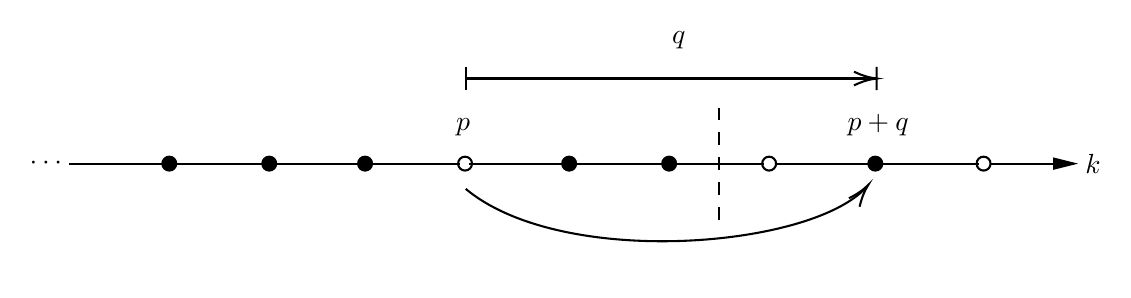
\begin{tikzpicture}[x=0.75pt,y=0.75pt,yscale=-1,xscale=1]
%uncomment if require: \path (0,300); %set diagram left start at 0, and has height of 300

%Straight Lines [id:da4100443293723468] 
\draw    (120,122) -- (168.17,122) ;
\draw [shift={(168.17,122)}, rotate = 0] [color={rgb, 255:red, 0; green, 0; blue, 0 }  ][fill={rgb, 255:red, 0; green, 0; blue, 0 }  ][line width=0.75]      (0, 0) circle [x radius= 3.35, y radius= 3.35]   ;
%Straight Lines [id:da8268118303886198] 
\draw    (168.17,122) -- (216.33,122) ;
\draw [shift={(216.33,122)}, rotate = 0] [color={rgb, 255:red, 0; green, 0; blue, 0 }  ][fill={rgb, 255:red, 0; green, 0; blue, 0 }  ][line width=0.75]      (0, 0) circle [x radius= 3.35, y radius= 3.35]   ;
%Straight Lines [id:da43623564624457467] 
\draw    (214.33,122) -- (262.5,122) ;
\draw [shift={(262.5,122)}, rotate = 360] [color={rgb, 255:red, 0; green, 0; blue, 0 }  ][fill={rgb, 255:red, 0; green, 0; blue, 0 }  ][line width=0.75]      (0, 0) circle [x radius= 3.35, y radius= 3.35]   ;
%Straight Lines [id:da6308249389864167] 
\draw    (312.67,122) -- (360.83,122) ;
\draw [shift={(360.83,122)}, rotate = 0] [color={rgb, 255:red, 0; green, 0; blue, 0 }  ][fill={rgb, 255:red, 0; green, 0; blue, 0 }  ][line width=0.75]      (0, 0) circle [x radius= 3.35, y radius= 3.35]   ;
%Straight Lines [id:da8842593044005784] 
\draw    (360.83,122) -- (409,122) ;
\draw [shift={(409,122)}, rotate = 0] [color={rgb, 255:red, 0; green, 0; blue, 0 }  ][fill={rgb, 255:red, 0; green, 0; blue, 0 }  ][line width=0.75]      (0, 0) circle [x radius= 3.35, y radius= 3.35]   ;
%Straight Lines [id:da5662220510723945] 
\draw    (511.33,122) -- (557.5,122) ;
%Straight Lines [id:da1025885832172786] 
\draw    (264.5,122) -- (308.32,122) ;
\draw [shift={(310.67,122)}, rotate = 0] [color={rgb, 255:red, 0; green, 0; blue, 0 }  ][line width=0.75]      (0, 0) circle [x radius= 3.35, y radius= 3.35]   ;
%Straight Lines [id:da2625028833353278] 
\draw [fill={rgb, 255:red, 255; green, 255; blue, 255 }  ,fill opacity=1 ]   (409,122) -- (454.82,122) ;
\draw [shift={(457.17,122)}, rotate = 0] [color={rgb, 255:red, 0; green, 0; blue, 0 }  ][line width=0.75]      (0, 0) circle [x radius= 3.35, y radius= 3.35]   ;
%Straight Lines [id:da640047666926592] 
\draw  [dash pattern={on 4.5pt off 4.5pt}]  (433.08,94.98) -- (433.08,149.02) ;
%Straight Lines [id:da04769096870790679] 
\draw    (460.17,122) -- (508.33,122) ;
\draw [shift={(508.33,122)}, rotate = 0] [color={rgb, 255:red, 0; green, 0; blue, 0 }  ][fill={rgb, 255:red, 0; green, 0; blue, 0 }  ][line width=0.75]      (0, 0) circle [x radius= 3.35, y radius= 3.35]   ;
%Straight Lines [id:da2262005685906321] 
\draw    (563.5,122) -- (604,122) ;
\draw [shift={(606,122)}, rotate = 180] [fill={rgb, 255:red, 0; green, 0; blue, 0 }  ][line width=0.08]  [draw opacity=0] (12,-3) -- (0,0) -- (12,3) -- cycle    ;
%Straight Lines [id:da032777578830224474] 
\draw    (514.33,122) -- (558.15,122) ;
\draw [shift={(560.5,122)}, rotate = 0] [color={rgb, 255:red, 0; green, 0; blue, 0 }  ][line width=0.75]      (0, 0) circle [x radius= 3.35, y radius= 3.35]   ;
%Curve Lines [id:da9438600897735019] 
\draw    (311,134.17) .. controls (357.3,172.75) and (477.33,162.65) .. (503.85,133.51) ;
\draw [shift={(505,132.17)}, rotate = 488.51] [color={rgb, 255:red, 0; green, 0; blue, 0 }  ][line width=0.75]    (10.93,-3.29) .. controls (6.95,-1.4) and (3.31,-0.3) .. (0,0) .. controls (3.31,0.3) and (6.95,1.4) .. (10.93,3.29)   ;
%Straight Lines [id:da4803509024076933] 
\draw    (509,81) -- (311,81) ;
\draw [shift={(311,81)}, rotate = 360] [color={rgb, 255:red, 0; green, 0; blue, 0 }  ][line width=0.75]    (0,5.59) -- (0,-5.59)   ;
\draw [shift={(509,81)}, rotate = 180] [color={rgb, 255:red, 0; green, 0; blue, 0 }  ][line width=0.75]    (0,5.59) -- (0,-5.59)(10.93,-3.29) .. controls (6.95,-1.4) and (3.31,-0.3) .. (0,0) .. controls (3.31,0.3) and (6.95,1.4) .. (10.93,3.29)   ;

% Text Node
\draw (118,122) node [anchor=east] [inner sep=0.75pt]   [align=left] {$\displaystyle \cdots $};
% Text Node
\draw (608,122) node [anchor=west] [inner sep=0.75pt]    {$k$};
% Text Node
\draw (309.67,110) node [anchor=south] [inner sep=0.75pt]    {$p$};
% Text Node
\draw (509.67,110) node [anchor=south] [inner sep=0.75pt]    {$p+q$};
% Text Node
\draw (409,57) node [anchor=north west][inner sep=0.75pt]    {$q$};


\end{tikzpicture}

    }
    \caption{右模式的玻色化}
\end{figure}

首先考虑右模式的电子。
按照\eqref{eq:one-dimension-linear-model},对一个能量本征态,将一个动量为$p$的右模式电子变为动量为$p+q$的右模式电子,则得到的结果仍然是一个能量本征态,且能量上升了$v_\text{F} q$。
而由于粒子数守恒,实际上任何一个能量本征态都可以通过“让费米海中的一些电子的动量增加”构造出来。这表明“将一个动量为$p$的右模式电子变为动量为$p+q$的右模式电子”是一个准粒子模式,其产生算符大体上如下:
\[
    {b}_{\text{R} q}^\dagger \sim \sum_p {c}^\dagger_{\text{R} (p+q)} {c}_{\text{R} p} ,
\]
但是这样$p$可以取任何大的值,而低能有效理论\eqref{eq:one-dimension-linear-model}仅仅对比较小的$p$成立。
因此不出意外会产生一个发散的问题。例如,按照\eqref{eq:one-dimension-linear-model}费米海中实际上有无限多的电子,从而不受限制的对$p$求和会导致无穷大的结果。
可以在${b}_{\text{R} q}^\dagger$的表达式中引入一个截断,但是更好的做法实际上是使用正规排序,从而将无穷大的电子数期望值去掉。我们接下来讨论怎么做到这一点。
实空间的电子数密度算符为
\[
    {\rho}_\text{R}(x) = {\psi}_\text{R}^\dagger(x) {\psi}_\text{R}(x),
\]
它在动量空间的形式为%
\footnote{它不一定就是动量为$p$的电子数。}%
\[
    {\rho}_\text{R}(p) = \frac{1}{\sqrt{L}} \int \dd{x} \ee^{-\ii p x} {\rho}_\text{R}(x) = \frac{1}{\sqrt{L}} \sum_k {c}^\dagger_{\text{R} (k - p)} {c}_{\text{R} k}.
\]
可以看到这个表达式和${b}^\dagger_{\text{R} p}$之间有线性关系,既然电子数在没有截断时发散,${b}^\dagger_{\text{R} p}$必然也发散。
为了消除掉发散,我们将${\psi}_\text{R}^\dagger(x) {\psi}_\text{R}(x)$的基态期望值减掉,得到下面的定义。这里使用了正规序的记号是因为这个步骤等价于以电子/空穴的产生算符为产生算符,换而言之,对费米面以下的电子,要把电子湮灭算符放在左边(或者说把空穴产生算符放在左边):
\begin{equation}
    {\rho}_\text{R}(x) = \normalorder{{\psi}_\text{R}^\dagger(x) {\psi}_\text{R}(x)}, \quad {\rho}_\text{R}(p) = \frac{1}{\sqrt{L}} \sum_k \normalorder{{c}^\dagger_{\text{R} (k - p)} {c}_{\text{R} k}}.
\end{equation}
然后很容易验证,在基态(即所有电子都在费米海中的状态)下${\rho}_\text{R}(p)$为零,这样就避免了无穷大问题。
计算对易关系得到
\[
    \comm*{{\rho}_\text{R}(- p)}{{\rho}_\text{R}(p)} = \frac{1}{L} \sum_{k} ({c}^\dagger_{\text{R} (k + p)} {c}_{\text{R} (k + p)} - {c}^\dagger_{\text{R} k} {c}_{\text{R} k}),
\]
此时不能简单地做变量代换,因为求和实际上带有一个截断,做变量代换则截断也会发生变化。
考虑到
\[
    \normalorder{{c}^\dagger_{\text{R} k} {c}_{\text{R} k}} = {c}^\dagger_{\text{R} k} {c}_{\text{R} k} - \expval*{{c}^\dagger_{\text{R} k} {c}_{\text{R} k}}_\text{GS},
\]
而正规序无需截断(因为没有发散问题),可以推导出
\[
    \comm*{{\rho}_\text{R}(- p)}{{\rho}_\text{R}(p)} = \frac{1}{L} \sum_{k} (\expval*{{c}^\dagger_{\text{R} (k + p)} {c}_{\text{R} (k + p)}}_\text{GS} - \expval*{{c}^\dagger_{\text{R} k} {c}_{\text{R} k}}_\text{GS}),
\]
等式右边的求和号中非零部分满足
\[
    k < 0 < k + p,
\]
并做通常的求和化积分
\[
    \frac{1}{L} \sum_k \longrightarrow \int \frac{\dd{k}}{2\pi},
\]
就得到
\[
    \comm*{{\rho}_\text{R}(- p)}{{\rho}_\text{R}(p)} = - \frac{p}{2\pi}.
\]
而如果$p \neq p'$,应有
\[
    \comm*{{\rho}_\text{R}(- p)}{{\rho}_\text{R}(p')} = 0,
\]
因为依照上面的步骤会得到的真空期望值一定是零。于是得到
\begin{equation}
    \comm*{{\rho}_\text{R}(- p)}{{\rho}_\text{R}(p')} = - \frac{p}{2\pi} \delta_{pp'}.
\end{equation}
这几乎就是一个玻色子对易关系了。缩放一下,定义
\begin{equation}
    {b}_{\text{R} p} = \sqrt{\frac{2\pi}{p}} {\rho}_\text{R}(p), \quad {b}^\dagger_{\text{R} p} = \sqrt{\frac{2\pi}{p}} {\rho}_\text{R}(-p),
    \label{eq:one-dim-displacement-mode}
\end{equation}
就得到了一组玻色子产生湮灭算符,它们描述的玻色子就是“将一个动量为$q$的右模式电子变为动量为$p+q$的右模式电子”这种模式。

以上讨论的都是右模式。由于动量空间左右对称,在变换
\[
    p \longrightarrow -p, \quad \text{R} \longrightarrow \text{L}
\]
下物理规律不变,于是只需要在每个关于右模式的公式中做以上代换就得到了关于左模式的公式。

容易检验可以从基态不断作用\eqref{eq:one-dim-displacement-mode}中的产生算符而获得一组基矢量,从而哈密顿量可以改写成
\begin{equation}
    {H} = \sum_{p > 0} v_\text{F} p \left({b}_{\text{R} p}^\dagger {b}_{\text{R} p} + {b}_{\text{L} -p}^\dagger {b}_{\text{L} -p} \right),
    \label{eq:one-dim-displacement-hamiltonian}
\end{equation}
其中我们忽略了一个无关紧要的能量零点变化。

\subsection{玻色子场论}

现在我们需要反过来做正则量子化:在已经找到了一种准粒子的产生湮灭算符之后,分析这个准粒子满足怎么样的一个场论。
定义
\begin{equation}
    {\phi}_\text{R}(p) = \frac{2\pi}{\ii p} {\rho}_\text{R}(p),
    \label{eq:one-dim-phi}
\end{equation}
切换到坐标空间中就是
\[
    {\rho}_\text{R}(x) = \frac{1}{2\pi} \grad \phi_\text{R}(x).
\]
如果用傅里叶变换证明这个关系,需要如下做傅里叶变换:
\begin{equation}
    {\phi}_\text{R} (x) = \frac{1}{\sqrt{L}} \sum_p \ee^{- \alpha \abs{p} / 2} \phi_\text{R}(p) \ee^{\ii p x} = \frac{1}{\sqrt{L}} \sum_p \ee^{- \alpha \abs{p} / 2} \frac{2\pi}{\ii p} {\rho}_\text{R}(p) \ee^{\ii p x},
    \label{eq:one-dim-phi-and-rho}
\end{equation}
其中$\alpha$为一个软截断。一维系统中的傅里叶变换有时会发散,需要手动压低。

定义
\begin{equation}
    \begin{cases}
        {\phi}_\text{R} = {\phi} + {\theta}, \\
        {\phi}_\text{L} = {\phi} - {\theta},
    \end{cases}
\end{equation}
通过傅里叶变换和${\rho}$的对易关系可以得到
\begin{equation}
    \comm*{{\phi}(x')}{\grad {\theta}(x)} = -\ii \pi \delta(x' - x).
\end{equation}
因此$\phi$和$- \grad{\theta} / \pi$是一对正则变量,可以尝试构造一个关于它们的场论。

回顾哈密顿量\eqref{eq:one-dim-displacement-hamiltonian},将\eqref{eq:one-dim-phi}和\eqref{eq:one-dim-displacement-mode}代入其中,得到
\[
    {H} = \pi v_\text{F} \sum_p \left( {\rho}_\text{R}(-p) {\rho}_\text{R}(p) + {\rho}_\text{L}(-p) {\rho}_\text{L}(p) \right).
\]
将\eqref{eq:one-dim-phi-and-rho}代入上式,得到
\begin{equation}
    H = \frac{v_\text{F}}{2\pi} \int \dd{x} \left( (\grad{\phi})^2 + (\grad{\theta})^2 \right).
\end{equation}
至此我们将一维自由系统的哈密顿量写成了关于连续玻色场$\phi$和$\theta$的形式,完成了玻色化。

实际上,一维系统中处理相互作用反而是比较容易的。事实上很大一类有相互作用的体系经过玻色化之后也会得到同样的表达式
\begin{equation}
    H = \frac{v_\text{F}}{2\pi} \int \dd{x} \left( \frac{1}{K} (\grad{\phi})^2 + K (\grad{\theta})^2 \right),
    \label{eq:one-dim-bosonization-hamiltonian}
\end{equation}
其中$K$称为Luttinger参数。
我们在分析费米液体时,曾经论证过一般来说密度-密度相互作用是重要的相互作用通道。考虑一个满足这一条件的一维电子系统,排斥性的密度-密度相互作用或者说前向散射为
\begin{equation}
    {H}_\text{int} = \frac{U}{2} \int \dd[3]{\vb*{r}} ({\rho}_\text{R}(\vb*{r}) + {\rho}_\text{L}(\vb*{r})) ({\rho}_\text{R}(\vb*{r}) + {\rho}_\text{L}(\vb*{r})),
\end{equation}
如果我们将这样一个相互作用加在二维及以上的电子系统中就得到了一个费米液体。在一维情况中,考虑到\eqref{eq:one-dim-phi},就得到
\begin{equation}
    {H}_\text{int} = \frac{U}{2\pi^2} \int \dd[3]{\vb*{r}} (\grad{\phi})^2.
\end{equation}
做修正
\begin{equation}
    v_\text{F}' = v_\text{F} \sqrt{1 + \frac{U v_\text{F}}{\pi}}, \quad K = \left( 1 + \frac{U v_\text{F}}{\pi} \right)^{- \frac{1}{2}},
\end{equation}
就得到了\eqref{eq:one-dim-bosonization-hamiltonian}。这也可以看成重整化导致参数跑动的一个平凡的例子。
\eqref{eq:one-dim-bosonization-hamiltonian}描述的系统称为\concept{Luttinger液体},它不是费米液体。
我们相信它不是费米液体的理由见下一节。

\subsection{路径积分表述}

对\eqref{eq:one-dim-bosonization-hamiltonian}做勒让德变换,在虚时间下做路径积分,得到
\[
    \begin{aligned}
        Z &= \int \fd{\theta} \fd{\phi} \exp(- \int \dd{\tau} \int \dd{x} \frac{1}{\ii} (- \grad{\theta} / \pi) \partial_\tau \phi + \frac{v_\text{F}}{2\pi} \left( \frac{1}{K} (\grad{\phi})^2 + K (\grad{\theta})^2 \right) ) \\
        &= \int \fd{\theta} \fd{\phi} \exp(- \int \dd{\tau} \int \dd{x} \frac{\ii}{\pi} \grad{\theta} \partial_\tau \phi + \frac{v_\text{F}}{2\pi} \left( \frac{1}{K} (\grad{\phi})^2 + K (\grad{\theta})^2 \right) ).
    \end{aligned}
\]
指数中的第一项实际上给出了一个Berry相。通过将指数中的内容配方,可以得到一个标准的高斯积分,将含$\theta$的部分积掉,得到(略去了积掉$\theta$之后剩下的一个常数因子)
\begin{equation}
    \mathcal{L} = \frac{1}{2\pi v_\text{F} K} \left( (\partial_\tau \phi)^2 + v_\text{F}^2 (\grad{\phi})^2 \right) , \quad Z = \int \fd{\phi} \exp(- \int \dd{\tau} \int \dd{x} \mathcal{L} ).
\end{equation}
做长度单位变换
\[
    \frac{x}{v_\text{F}} \longrightarrow x,
\]
就得到
\begin{equation}
    \mathcal{L} = \frac{1}{2\pi K} \left( (\partial_\tau \phi)^2 + (\grad{\phi})^2 \right).
    \label{eq:one-dim-scaleless-lag}
\end{equation}
实际上,$\theta$和$\phi$是对偶的,因为在变换
\[
    \phi \longleftrightarrow \theta, \quad K \longleftrightarrow \frac{1}{K}
\]
下系统不变。因此完全可以将$\phi$积掉而留下$\theta$。

考虑一个简单的例子来展示为什么Luttinger液体不是费米液体。
在长波极限下,有
\begin{equation}
    {\psi}_\text{L} \sim \ee^{\ii \phi_\text{L}(x)}.
\end{equation}
容易验证至少上式两边和${\psi}^\dagger_\text{R}$的对易关系一致。
这样,
\[
    \expval*{{\psi}_\text{R}^\dagger(x) {\psi}_\text{R}(0)} = \expval*{\ee^{\ii ({\theta}(0) + {\phi}(0) - {\theta}(x) - {\phi}(x))}}.
\]
由于是自由场,通过Wick定理可以发现
\[
    \expval{\ee^{{A}}} = \ee^{\frac{1}{2} \expval*{{A}^2}},
\]
于是
\[
    \expval*{{\psi}_\text{R}^\dagger(x) {\psi}_\text{R}(0)} = \exp(- \frac{1}{2} \expval{({\theta}(0) + {\phi}(0) - {\theta}(x) - {\phi}(x))^2}).
\]
不失一般性地认为$\tau=0$,并注意到系统在变换
\[
    \tau \longrightarrow - \tau, \quad \theta \longrightarrow -\theta
\]
下不变,于是
\[
    \expval*{{\theta}(x, 0) {\phi}(x, 0)} = \expval*{- {\theta}(x, 0) {\phi}(x, 0)},
\]
即
\[
    \expval*{{\theta}(x, 0) {\phi}(x, 0)} = 0.
\]
因此
\[
    \expval*{{\psi}_\text{R}^\dagger(x) {\psi}_\text{R}(0)} = \exp(- \frac{1}{2} \expval{({\theta}(0) - {\theta}(x))^2}) \exp(- \frac{1}{2} \expval{({\phi}(0) - {\phi}(x))^2}).
\]
我们考虑接近零温的情况,此时\eqref{eq:one-dim-scaleless-lag}可以写成
\[
    \mathcal{L} = \sum_{\omega_n, k} \frac{K}{2\pi} \theta^*(k, \omega_n) (\omega_n^2 + k^2) \theta(k, \omega_n) = \sum_{\omega_n, k} \frac{1}{2\pi K} \phi^*(k, \omega_n) (\omega_n^2 + k^2) \phi(k, \omega_n),
\]
于是
\[
    \expval*{{\theta}^\dagger(k, \omega_n) {\theta}(k, \omega_n)} = \frac{\pi}{K (\omega_n^2 + k^2)}, \quad \expval*{{\phi}^\dagger(k, \omega_n) {\phi}(k, \omega_n)} = \frac{\pi K}{\omega_n^2 + k^2}.
\]
通过傅里叶逆变换得到
\[
    \frac{1}{2} \expval{({\theta}(0) - {\theta}(x))^2} = \frac{\pi}{k} \int \frac{\dd{k} \dd{\theta}}{(2\pi)^2} \frac{1 - \ee^{\ii k x \cos \theta}}{k} \sim \frac{1}{2K} \ln x, \quad \abs*{x} \gg 1.
\]
最后就可以得到
\[
    \expval*{{\psi}_\text{R}^\dagger(x) {\psi}_\text{R}(0)} \sim \abs*{x}^{-\frac{1}{2}(K + \frac{1}{K})}.
\]
做傅里叶逆变换,得到$k$很小时的动量分布函数
\[
    \expval{{n}_k} \sim \abs*{k}^{\frac{1}{2}(K + \frac{1}{K}) - 1}.
\]
如果$K=1$,上式右边有一个奇异性,这是费米液体的特征,因为费米面处电子数有一个跳变;但$K \neq 1$时上式右边是光滑的。这就说明了有相互作用的一维电子系统不是费米液体。

\subsection{玻色化导致共形场论}

一维自由电子系统和有前向散射的电子系统的低能自由度是Luttinger液体,这件事是已经确定的、完全物理的结果。
注意到

\subsection{自旋-电荷分离}

做变换
\begin{equation}
    \phi_{\text{charge}} = \frac{1}{\sqrt{2}} (\phi_\uparrow + \phi_\downarrow), \quad \phi_{\text{spin}} = \frac{1}{\sqrt{2}} (\phi_\uparrow - \phi_\downarrow),
\end{equation}
注意到由于$\phi \sim n$,如其下标所暗示的那样,$\phi_\text{charge}$和电荷密度涨落正相关而$\phi_\text{spin}$和$z$方向上的自旋密度涨落正相关。
因此实际上我们的体系中有两种彼此解耦的密度波,它们分别是自旋密度波和电荷密度波,两者的运行速度还不一样。
这是\concept{自旋电荷分离},是\concept{分数化激发}的一个典型例子,即强关联系统中作为基质的粒子携带一些标签,对称性等保证了这些标签在系统的元激发中一定会保留下来,但是未必在同一种激发上,使得这些标签似乎分开了。

\section{一维t-J模型}

\subsection{一维t-J模型和sine-Gordon模型}

一维情况下,t-J模型中的格点可以使用一个整数标记,即
\begin{equation}
    H = - t \sum_{i, \sigma} c_{i \sigma}^\dagger c_{i+1, \sigma} + \text{h.c.} + J \sum_i (\vb*{S}_i \cdot \vb*{S}_{i+1} - n_i n_{i+1} / 4).
\end{equation}
在做完玻色化之后,我们会发现其电荷密度波部分由一个$U(1)$自由模型描述,而其自旋密度波部分由一个$SU(2)$的sine-Gordon模型描述。
\begin{equation}
    H = H_\text{c} + H_\text{s} + \frac{2g_1}{(2\pi \alpha)^2} \int \dd{x} \cos(\sqrt{8} \phi_\text{s}),
\end{equation}
其中
\begin{equation}
    H_\nu = \frac{1}{2\pi}
\end{equation}
需注意自旋密度波部分的$SU(2)$对称性并没有体现在哈密顿量的形式中,而是体现在其参数满足的约束中,只有
\begin{equation}
    g_1 = K
\end{equation}
时才具有$SU(2)$对称性;这个约束正好是sine-Gordon模型的重整化群流中的两条斜对角的线。

sine-Gordon模型在$g_1$和$K$的不同安排下会落入两个相之一,其中之一的关联函数幂律衰减,对应无能隙的Luttinger液体,另一个的关联函数指数衰减,对应一个有能隙的系统。

\subsection{超导}

一维t-J模型既然是强关联系统,很容易想到,是否可能在其中寻找超导相。
本节利用玻色化计算超导序参量。我们有
\begin{equation}
    \Delta(x_i) = \psi_{i \uparrow} \psi_{i+1, \downarrow} - \psi_{i \downarrow} \psi_{i+1, \uparrow},
\end{equation}
用玻色化后得到的场表示,就有
\begin{equation}
    \begin{aligned}
        \Delta(x_i) &= \ee^{\ii (\theta_\uparrow + \theta_\downarrow + \phi_\uparrow + \phi_\downarrow + 2 k_\text{F} x_i)} + \ee^{\ii (\theta_\uparrow + \theta_\downarrow - \phi_\uparrow - \phi_\downarrow - 2 k_\text{F} x_i)} + \\
        &= 
    \end{aligned}
\end{equation}

\section{Hubbard模型的玻色化}

\section{海森堡模型的玻色化}